\subsection{Problemas}
--------------------------------------------------------
\\

\np
Dos varillas de longitud $L$ están a lo largo del eje $x$, una entre $x=a/2$ y $x=a/2+L$ y la otra entre $x=-a/2$ y $x=-a/2-L$. Cada varilla tiene carga positiva Q distribuida uniformemente.

\begin{enumerate}[label=\alph*)]
    \item Calcule el campo eléctrico producido por la segunda varilla en puntos a lo largo del eje $x$ positivo.
    \item Calcule la magnitud de la fuerza que ejerce una varilla sobre la otra.
\end{enumerate}

\np
\begin{enumerate}[label=\alph*)]
    \item Determine el campo eléctrico en todos los puntos del eje de un anillo de radio $R$ sobre el cual hay una densidad de carga uniforme $\lambda$.
    \item A partir de su resultado anterior, calcule el campo eléctrico creado por una corona circular de radios $R_1$ y $R_2$ ($R_1 < R_2$), sobre la cual hay una densidad de carga uniforme $\sigma$, en los puntos de su eje. Encuentre la magnitud y la dirección del campo eléctrico. Considere puntos arriba y abajo de la corona circular.
    \item ¿A qué se reduce su resultado si $R_1 \longrightarrow 0$? ¿Y si $R_2 \longrightarrow \infty$?
    \item Demuestre que en puntos sobre el eje de la corona (eje $z$) que estén suficientemente cerca del origen, la magnitud del campo eléctrico es aproximadamente proporcional a la distancia entre el centro de la corona circular y el punto. ¿Qué tan cerca es ”suficientemente cerca”?
\end{enumerate}

\np
\begin{enumerate}[label=\alph*)]
    \item Encuentre el campo eléctrico creado por un segmento rectilíneo de longitud $L$ dotado de una densidad de carga uniforme $\lambda$.
    \item A partir del resultado anterior, calcule el campo eléctrico en todos los puntos del espacio, producido por una línea infinita con densidad de carga $\lambda$.
    \item Calcule el flujo de campo eléctrico a través de una superficie cilíndrica cerrada, de largo h y radio R, concéntrica con la línea infinita.
    \item  Se tienen dos líneas infinitas con densidad de carga $\lambda$ y $-\lambda$, situadas a una distancia $2a$ una de la otra. Encuentre la fuerza por unidad de longitud que se establece entre los dos hilos. ¿Es atractiva o repulsiva?
\end{enumerate}
\newpage
\np
Considere un plano infinito (en las direcciones $x$ e $y$) de grosor $2R$ (en la dirección $z$), cargado con una densidad de carga volumétrica $\rho$ uniforme. Este plano tiene un agujero cilíndrico (cuyo eje coincide con el eje $y$) de radio $R$ sin cargas.
\begin{enumerate}[label=\alph*)]
    \item Determine el campo eléctrico en todo el espacio. Note que debería dividir el resultado en 3 zonas distintas.
    \item Calcule la fuerza que experimenta un alambre de largo $L$ con densidad de carga lineal uniforme $\lambda$ ubicado a una distancia $d$ del plano y extendido en la dirección $z$.
    \item Calcule la fuerza que experimenta un alambre de largo $L$ con densidad de carga lineal uniforme $\lambda$ ubicado a una distancia $d+L/2$ del plano y extendido en la dirección $y$.
\end{enumerate}

\begin{figure}[h]
    \centering
    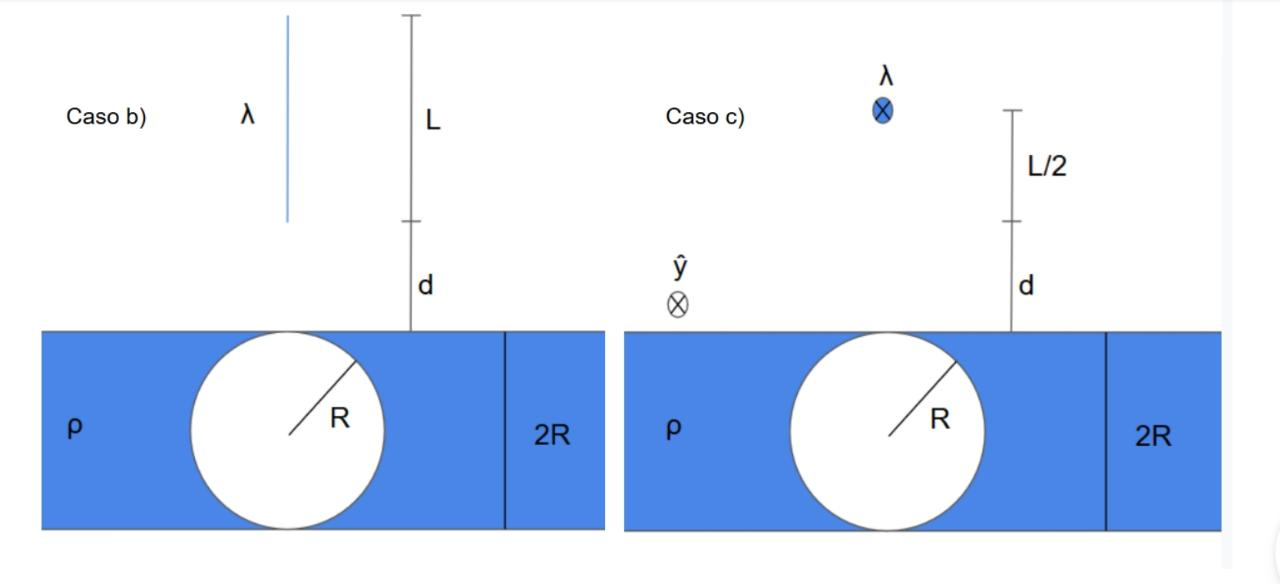
\includegraphics[width=0.9\textwidth]{Electroestática/Campo_electrico/P1 guia2 Mancilla.jpeg}
    \label{fig:P1G2M}
\end{figure}

\np
\begin{enumerate}[label=\alph*)]
    \item Si el campo eléctrico de una carga puntual fuera proporcional a $1/r^3$ en vez de $1/r^2$, ¿seguiría siendo válida la ley de Gauss? Explique su razonamiento. (Sugerencia: considere una superficie esférica centrada en una sola carga puntual).
    \item  Cierta región del espacio limitada por una superficie imaginaria cerrada no contiene carga. ¿El campo eléctrico siempre es igual a cero en todos los puntos de la superficie? Si no es así, ¿en qué circunstancias sería cero en la superficie?
    \item En cierta región del espacio, el campo eléctrico es uniforme. Use la ley de Gauss para demostrar que esa región debe ser eléctricamente neutra; es decir, la densidad volumétrica de carga $\rho$ debe ser igual a cero. Lo contrario, ¿es verdadero? Es decir, en una región del espacio donde no hay carga, ¿debe ser uniforme?
\end{enumerate}

\np
Imagine una esfera de radio R rellena con carga negativa de densidad uniforme y una carga total equivalente a la carga de dos electrones, es decir, $-2e$. En el interior de esta gelatina de carga negativa, se encuentran dos protones, cada uno de ellos de carga $e$. Asuma que, a pesar de la presencia de los protones, la distribución de carga negativa se mantiene uniforme. ¿Dónde deben ubicarse los protones de modo que la fuerza en cada uno de ellos sea nula? Para responder esta pregunta, siga estos pasos:
\begin{enumerate}[label=\alph*)]
    \item Calcule el campo eléctrico producido por los electrones.
    \item Calcule la fuerza de Coulomb neta sobre uno los protones.
    \item Determine la condición de equilibrio y concluya.
\end{enumerate}


\newpage